%%%%%%%%%%%%%%%%%%%%%%%%%%%%%%%%%%%%%%%%%%%%%%%%%%%%%%%%%%%%%%%%%%%%%%%%%%%%%%%


\chapter{EFEITOS DA JANELA DE OBSERVAÇÃO}

Os principais artefatos da análise espctral são o \textit{aliasing} e o \textit{spectral leakage}, ou vazamento espectral. Spectral leakage é o ``vazamento'' da energia devida a uma frequência existente no sinal para outras, por exemplo os lóbulos laterais presentes em muitos espectros. Aliasing é um tipo de leakage, que é o efeito do espectro apresentar assinaturas falsas de sinais (alias vem do inglês e significa pseudônimo), e será abordado na próxima seção. A figuras desta seção exemplificam os fenômenos de leakage e ilustram suas causas.

\begin{figure}[ht!]
	\caption{Efeitos da amostragem finita.}
	\vspace{1mm}	% acrescentar o espaçamento vertical apropriado entre o título e a borda superior da figura
	\begin{center}
		\resizebox{15cm}{!}{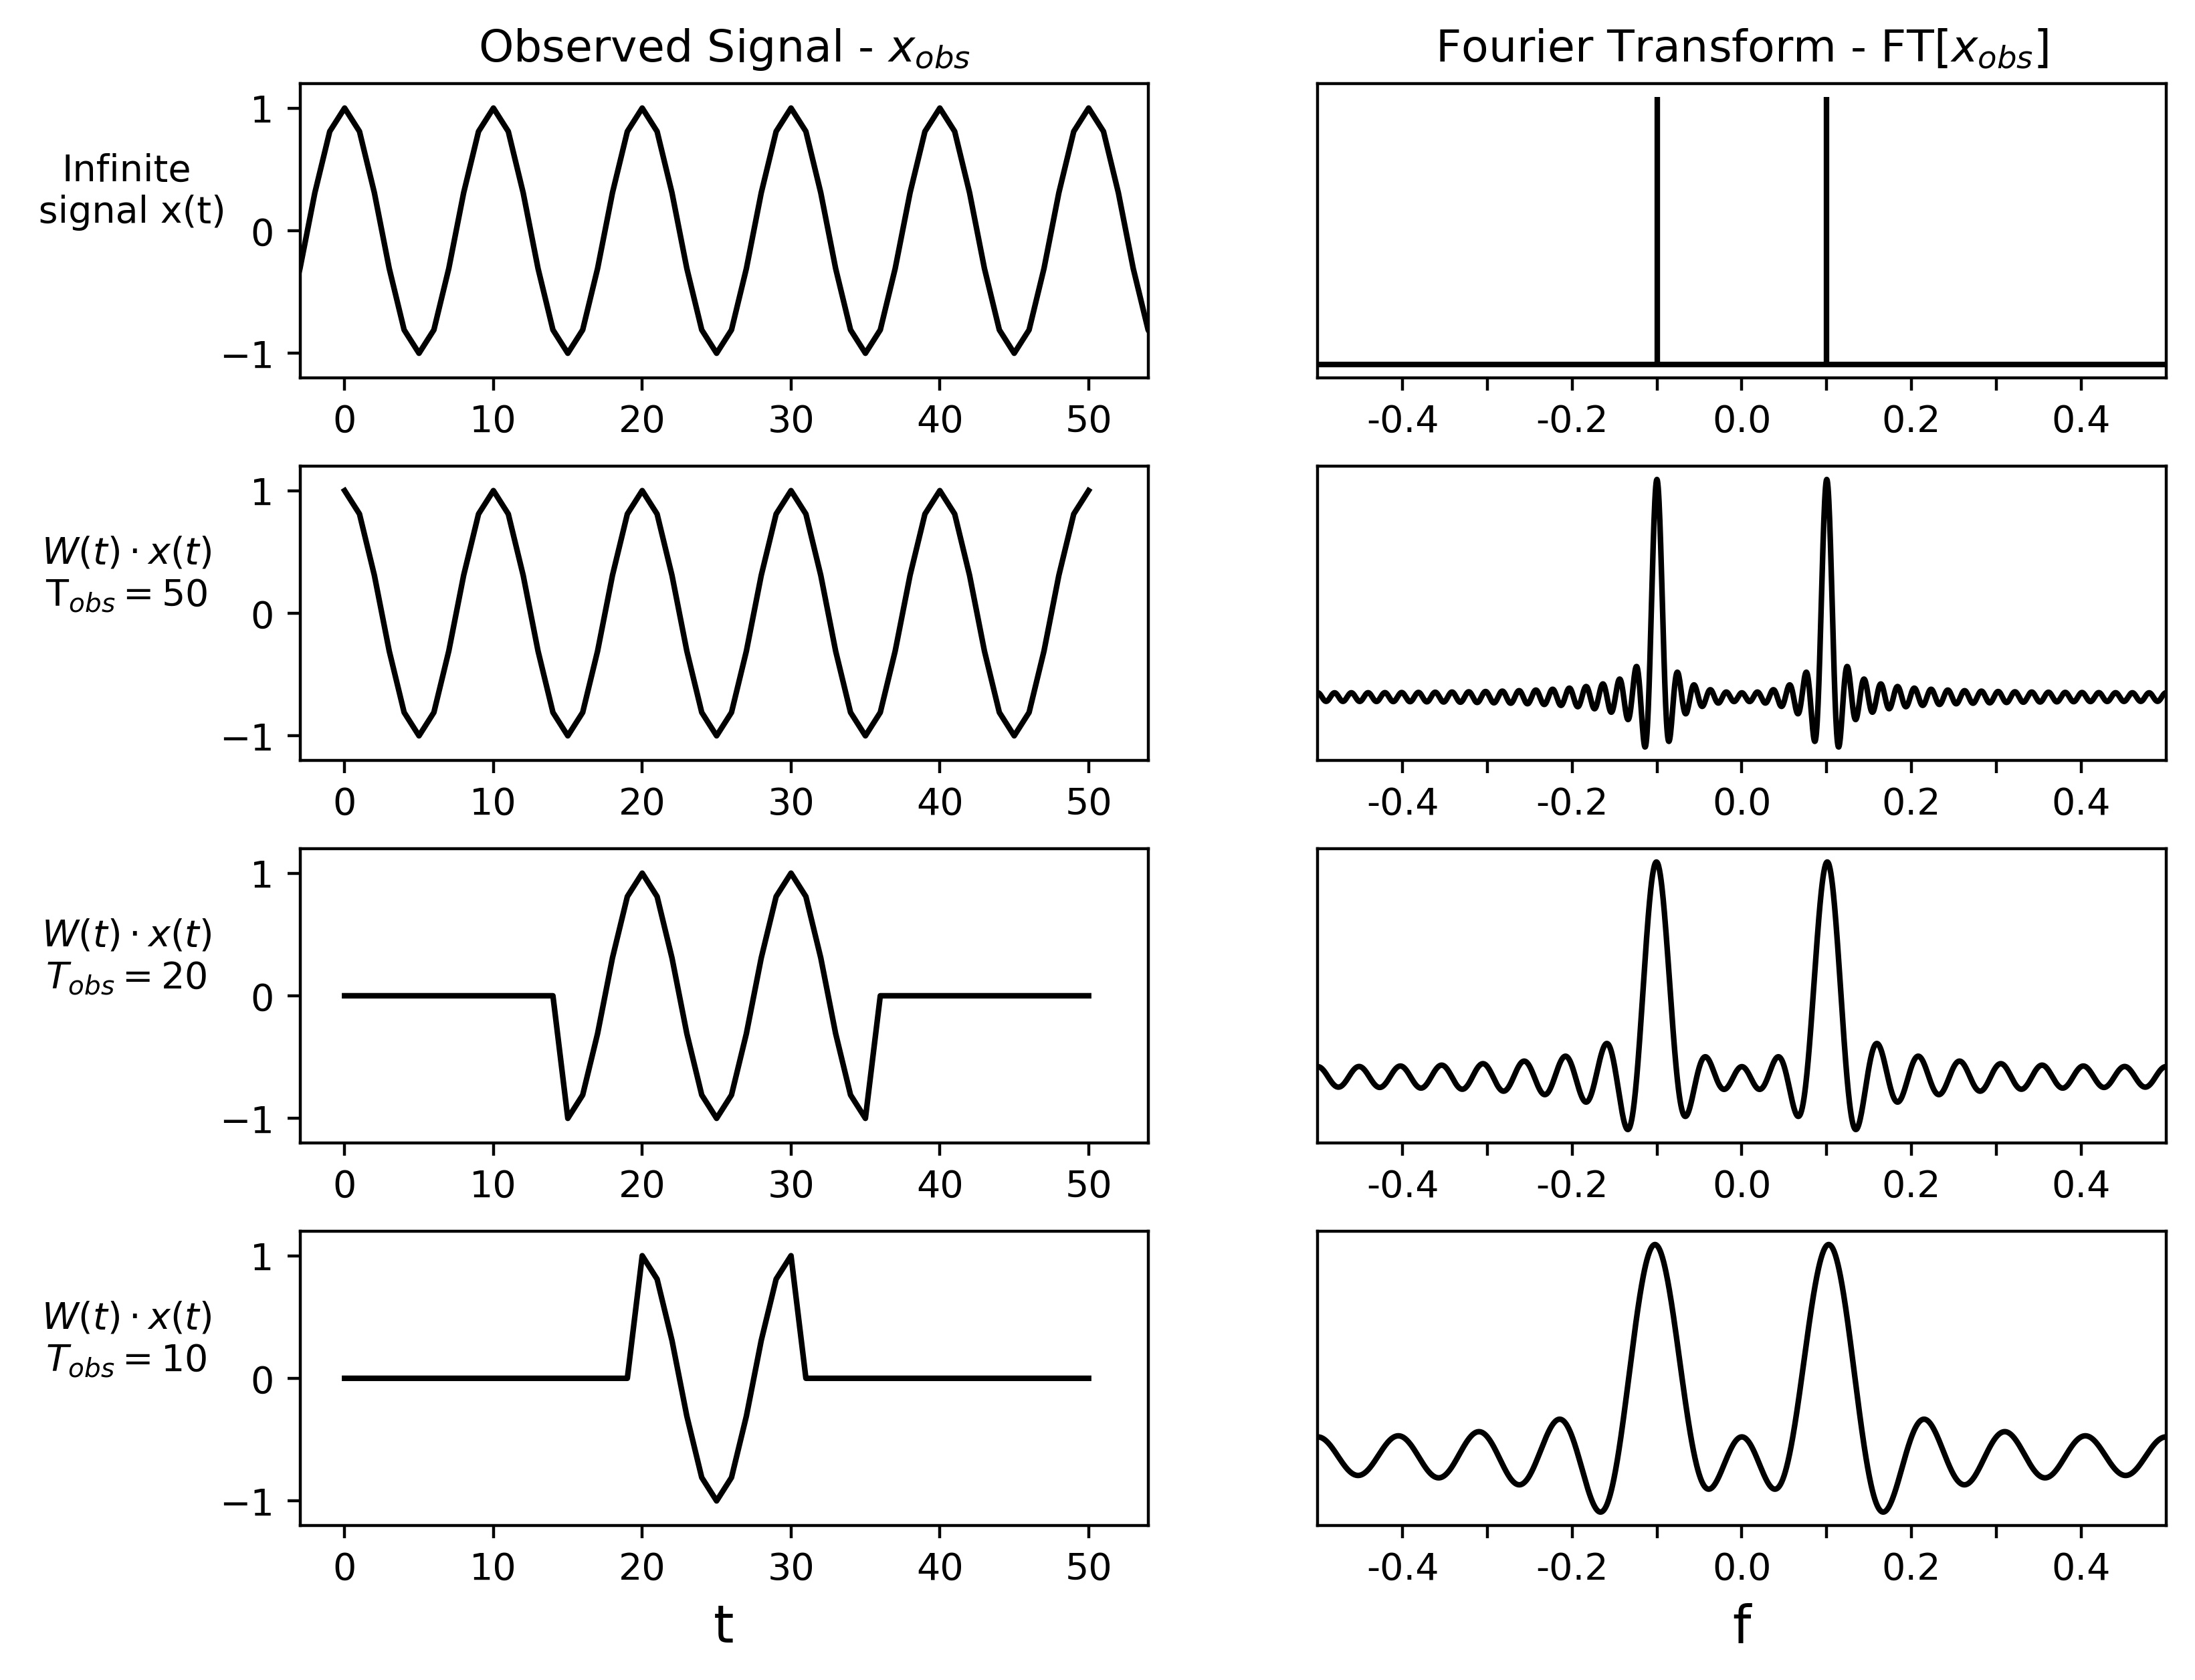
\includegraphics{Figuras/window.jpg}}
	\end{center}
	\vspace{1mm}	% acrescentar o espaçamento vertical apropriado entre a borda inferior da figura e a legenda ou a fonte quando não há legenda (o valor pode ser negativo para subir)
	\legenda{Efeitos do tamanho da janela de observação sobre a transformada de Fourier de um sinal. No topo à esquerda o sinal está representado por uma função analítica que se estende infinitamente, cuja transformada de Fourier (topo à direita) é a função delta sobre a frequência do sinal (no caso $f_{0} =$ 0.1). Abaixo estão sinais com janelas de observação diferentes e suas respectivas transformadas. Quanto menor a janela de observação, maior o efeito dos lóbulos laterais sobre a função delta original, o chamado leakage espectral, e menor a resolução da transformada (maior a largura da assinatura principal).}	% legenda - para deixar sem legenda usar comando \legenda{} (nunca deve-se comentar o comando \legenda)
	\label{fig:window}
	%\FONTE{\url{https://omniweb.gsfc.nasa.gov/form/dx1.html}.}	% fonte consultada (elemento obrigatório, mesmo que seja produção do próprio autor)
\end{figure}

\begin{figure}[ht!]
	\caption{Efeitos da amostragem finita.}
	\vspace{1mm}	% acrescentar o espaçamento vertical apropriado entre o título e a borda superior da figura
	\begin{center}
		\resizebox{15cm}{!}{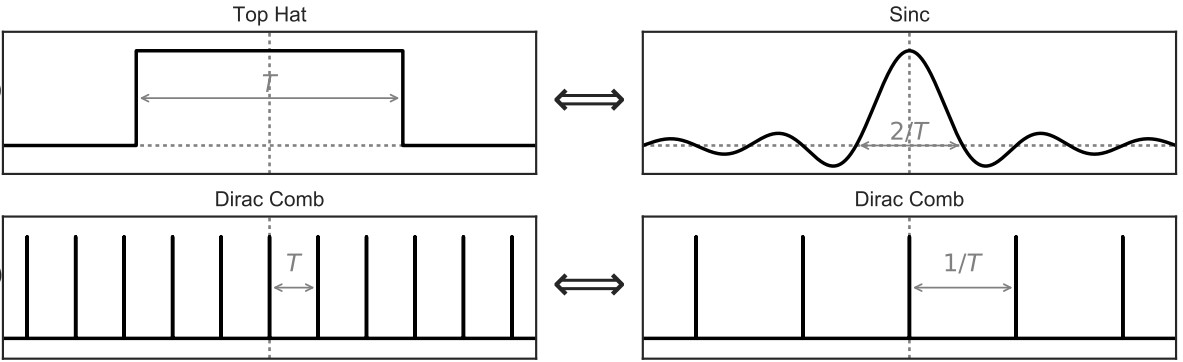
\includegraphics{Figuras/adaptado.jpg}}
	\end{center}
	\vspace{1mm}	% acrescentar o espaçamento vertical apropriado entre a borda inferior da figura e a legenda ou a fonte quando não há legenda (o valor pode ser negativo para subir)
	\legenda{Pares de transformada relevantes para esta seção. Nos gráficos de cima, a transformada de Fourier da função retangular (top hat) gera a função Sinc. Embaixo, a transformada de Fourier  de uma combinação de funções delta (espaçadas por um período $T$) gera outra combinação de funções delta (espaçadas por uma frequência $1/T$).}	% legenda - para deixar sem legenda usar comando \legenda{} (nunca deve-se comentar o comando \legenda)
	\label{fig:adaptado}
	\FONTE{Adaptado de \citeonline{2017arXiv170309824V}.}	% fonte consultada (elemento obrigatório, mesmo que seja produção do próprio autor)
\end{figure}


A coluna esquerda da Figura \ref{fig:window} pode ser entendida como sucessivos produtos da função do topo por janelas de observação cada vez menores, de modo que a análise não será mais feita sobre o sinal $x(t)$ (gerando a transformada do topo à direita), mas sim sobre um novo sinal:

\begin{equation}
x_{obs}(t) = x(t) \cdot W(t),
\label{eq:xobs}
\end{equation}
onde $W$ é a função janela (ou do inglês, \textit{window}) que multiplica o sinal original. Conforme o Teorema da Convolução, temos então

\begin{equation}
\text{FT}[x_{obs}] = \text{FT}[x(t)] \star \text{FT}[W(t)].
\end{equation}

O resultado desta convolução é a coluna da direita da Figura \ref{fig:window}. Quanto menor o tamanho da janela, os efeitos observados são dois: maior a largura da função representando a transformada, e maior a magnitude das oscilações próximas a $y=0$, os lóbulos laterais. As janelas de observação da figura são $T_{obs} = $ 50, 20 e 10. A transformada de cada uma dessas funções janela (ver par de transformada da linha de cima da Figura \ref{fig:adaptado}) confere à transformada de $x_{obs}$ suas características, uma vez que $x(t)$ é o mesmo sinal em todas as transformadas da figura.

De fato, a largura da FT na coluna da direita da Figura \ref{fig:window} é $\delta f \sim 1/T_{obs}$. Como a janela de observação do sinal do topo é infinita, sua transformada é a função delta (de largura zero). Já os lóbulos laterais vão a zero de maneira oscilatória (e periódica). Em outras palavras, há um vazamento para outras frequências. 

Pode-se resolver o problema do vazamento espectral ao definir uma função $W(t)$ que produza um corte gradual sobre o sinal de modo a eliminar o fim abrupto de informação nas fronteiras, ou seja, uma função que vá gradualmente a zero em $-T_{obs}/2$ e $T_{obs}/2$. Uma função muito usada é a função de Hanning, que reduz drasticamente os lóbulos laterais.



